\documentclass[11pt,a4paper]{article}
\usepackage[UTF8,heading=true]{ctex}
\usepackage[a4paper,left=25mm,right=25mm,top=22mm,bottom=22mm]{geometry}
\usepackage{fontspec,xeCJK,graphicx,booktabs,array,amsmath,amssymb}
\usepackage[hidelinks]{hyperref}
\setmainfont{Times New Roman}
\setCJKmainfont{SimSun}[BoldFont=SimHei]
\setCJKsansfont{SimHei}
\setlength{\parindent}{2em}
\setlength{\parskip}{3pt}
\linespread{1.18}
\setlength{\tabcolsep}{6pt}
\setlength{\abovecaptionskip}{5pt}
\emergencystretch=1.5em
\widowpenalty=10000\clubpenalty=10000
\ctexset{section={format=\Large\bfseries},subsection={format=\large\bfseries},subsubsection={format=\normalsize\bfseries}}
\graphicspath{{figures/}}
\makeatletter
\newcommand{\tableinput}[1]{\@@input #1 }
\newenvironment{inlinefigure}{\par\addvspace{8pt}\noindent\begin{minipage}{\linewidth}\def\@captype{figure}\centering}{\end{minipage}\par\addvspace{8pt}}
\newenvironment{inlinetable}{\par\addvspace{7pt}\noindent\begin{minipage}{\linewidth}\def\@captype{table}\centering\small}{\end{minipage}\par\addvspace{7pt}}
\makeatother
\setcounter{secnumdepth}{2}
\pagestyle{plain}
\begin{document}
\section*{问题二的模型建立与求解}
\subsection*{1\quad 未知供需下的日前购电安排}

问题一根据给定的一天供需曲线安排购电。问题二的困难在于，当天用多少电、光伏能发多少电，在零点都还没有发生，但普通购电量必须先确定。少买的部分可能要用五倍电价补购；多买的电若用不掉、也存不下，仍然需要付款。因此，本问要在提前多作准备的费用与临时补电的风险之间作出取舍。

为此，先分别估计负载和光伏，再根据过去的预测偏差增加适量准备，最后安排外网购电和储能。白天普通订单保持不变，电池按实际供需补缺或充电，剩余缺口才由紧急购电补齐。这样既沿用问题一的电量平衡和设备限制，又能反映提前订电与实际用电之间的差别。

\subsection*{2\quad 负载与光伏的分别预测}

负载的星期规律较强，光伏则更受近期发电水平影响。若只预测二者的差值，容易把不同来源的变化混在一起。因此，分别用同星期历史估计负载，用近期历史估计光伏。以 $d$ 表示自然日，$k=1,\ldots,144$ 表示日内时段，每段长 $\Delta t=1/6$ 小时，第1段从0:00开始，第144段到24:00结束。$L_{d,k}$、$V_{d,k}$ 分别为负载和光伏功率，单位为 kW。历史充足时，预测为
\begin{equation}
\widehat L_{d,k}=\frac14\sum_{j=1}^{4}L_{d-7j,k},\qquad
\widehat V_{d,k}=\frac17\sum_{j=1}^{7}V_{d-j,k}.
\label{eq:forecast}
\end{equation}
也就是说，负载参考过去四个相同星期的同一时刻，光伏参考最近七天的同一时刻。选中的负载历史各占四分之一，光伏历史各占七分之一。历史不足时按已有记录取平均；尚无可用记录的启动处理见第5节。

式\eqref{eq:forecast}只使用当天零点以前的数据。附件2虽然保存了全年实际值，但当天及其后的真实值不参与当天预测。本问也不使用附件3的光伏预报。后面规划中涉及次日时，负载改为匹配次日的星期，光伏仍参考当前零点之前的七天，不能提前读入当天实际发电。

\subsection*{3\quad 根据近期误差确定准备量}

平均预测给出了通常的供需水平，却未必能应对连续几段的低估。电池能够补一段缺口，连续补电后仍可能达到储电下限。为减少这种情况，考察过去究竟把缺口看小了多少，并将其作为订电的准备依据。

对过去日期 $i$，按该日零点可获得的信息重建预测，定义净供需误差
\begin{equation}
\epsilon_{i,k}=\big[(L_{i,k}-V_{i,k})-(\widehat L_{i,k}-\widehat V_{i,k})\big]\Delta t.
\label{eq:error}
\end{equation}
正值表示实际比预计更缺电，负值表示预计偏保守，单位均为 kWh。负载和光伏在预测时分开，在这里合并误差，是为了保留二者可能相互抵消、也可能共同扩大缺口的关系。

将一天分为六个4小时组，在最近28天中收集同组误差。较早的误差仍有参考价值，但近期供需已经改变时，不宜让旧记录占据同样分量。因此，对组内日期 $i$ 的每个时段赋予权重
\begin{equation}
\omega_{d,i,k}=\frac{\beta^{d-1-i}}
{\displaystyle\sum_{(j,u)\in\mathcal E_{d,g}}\beta^{d-1-j}},\qquad (i,k)\in\mathcal E_{d,g},
\label{eq:weight}
\end{equation}
其中，$\mathcal E_{d,g}$ 是当天零点以前、最近28天第 $g$ 组的误差集合。$\beta$ 控制旧记录的权重下降速度。取 $\beta=0.7$ 时，满28天历史中，最近三天的合计权重约为30\%、21\%和14.7\%；同一天同组内各时段等分该日权重。

再将误差从小到大排列，取加权累计比例达到 $\alpha$ 的位置，并将负值截为零。写成
\begin{align}
F_{d,g}(u)&=\sum_{(i,k)\in\mathcal E_{d,g}}\omega_{d,i,k}\,\mathbf{1}\{\epsilon_{i,k}\le u\},\\
b_{d,k}&=\max\left\{0,\inf\{u:F_{d,g(k)}(u)\ge\alpha\}\right\}.
\label{eq:margin}
\end{align}
$\mathbf1$ 在条件成立时取1，否则取0；$g(k)$ 表示时段 $k$ 所属的4小时组。采用 $\alpha=0.7$。它是误差排序的位置，与 $\beta$ 的时间权重含义不同，也不表示多买70\%的电或供电可靠率达到70\%。

准备量 $b_{d,k}$ 加在预测净需求上，由后续调度统一安排。它可能增加普通购电，也可能减少预计用于充电的光伏富余，或者改变电池放电时机，因而不是每段直接追加同样数量的订单。负误差也参与排序，避免只保留缺电记录而把准备量系统性抬高。

\subsection*{4\quad 购电与储能调度模型}

\textbf{决策变量。} 为兼顾午夜之后的用电，每天零点向前规划48小时，共288段，仅固定当天前144段的普通订单。以下以 $t$ 表示这两天中连续排列的时段。先由预测和准备量算出
\begin{equation}
r_t=(\widehat L_t-\widehat V_t)\Delta t+b_t,\qquad
n_t=\max(r_t,0),\quad a_t=\max(-r_t,0).
\end{equation}
$n_t$ 是需要外网或电池补充的电量，$a_t$ 是考虑准备量后预计可用于储存的富余。二者都是给定量。令 $x_t$ 为外网用于充电的电量，$y_t$ 为光伏用于充电的电量，$z_t$ 为电池送给负载的电量，$S_t$ 为段末内部储电量。前三者按设备外侧计量，$S_t$ 按内部计量，单位均为 kWh。普通订单为
\begin{equation}
q_t=n_t-z_t+x_t.
\label{eq:order}
\end{equation}
式\eqref{eq:order}表示：剩余负载先扣除电池能提供的部分，再加上主动购买的充电电量。外网可以直接供负载，也可以在低价时为电池充电。

\textbf{目标函数。} 计划费用按固定日内电价 $p_t$ 计算，两个规划日重复使用同一电价曲线。为给规划期末的余电保留一个未来使用的参考价值，目标取为
\begin{equation}
\min\ J=\sum_{t=1}^{288}p_tq_t-\nu S_{288},\qquad
\nu=0.9p_{00:00}=0.38484.
\label{eq:objective}
\end{equation}
内部1 kWh电量最多向负载输出0.9 kWh，因此用0.9倍参考电价估计其价值。该项只帮助比较计划，不是售电收入，最终费用中不扣除它。真实的紧急购电尚不可知，这里以误差准备量应对其风险；方案好坏仍按实际发生的普通与紧急电费评价。

\textbf{约束条件。} 充电和放电效率各为90\%，储电量按
\begin{equation}
S_t=S_{t-1}+0.9(x_t+y_t)-\frac{z_t}{0.9},\qquad
1200\le S_t\le10800
\label{eq:storage}
\end{equation}
逐段衔接。充入100 kWh，内部增加90 kWh；若向负载送出90 kWh，内部需减少100 kWh。充放电量还须满足
\begin{equation}
\begin{aligned}
&x_t\ge0,\qquad 0\le y_t\le a_t,\qquad q_t\ge0,\\
&x_t+y_t\le5000\Delta t,\qquad
0\le z_t\le\min\{n_t,5000\Delta t\},\quad t=1,\ldots,288.
\end{aligned}
\label{eq:bounds}
\end{equation}
这里的5000 kW是电池的充、放电功率限制，换成10分钟电量后，每段外侧充电或放电最多833.33 kWh。$y_t\le a_t$ 防止储存不存在的光伏富余，$z_t\le n_t$ 防止向负载送出超过其需求的电。

$S_0$ 取当天实际剩余电量，不再要求每天首尾相等。给定预测与准备量后，式\eqref{eq:order}--\eqref{eq:bounds}构成连续线性规划，使用 HiGHS 求解。正电价下，同时用外网充电又向负载放电只会多付转换损耗，最优计划可避免这种动作；保存的求解结果也未出现同段同时充放。线性规划的最优性针对给定预测下的计划，并不等于已知未来真实供需时的最低全年电费。

\subsection*{5\quad 每日求解、实际供电与跨日运行}

每天零点先更新历史数据和电池库存，依次求出预测、准备量及普通订单。白天按10分钟区间检查实际供需。设本段负载和光伏电量为 $l$、$v$，按光伏优先直供的运行假设，直供量为 $m=\min(l,v)$，剩余负载为 $h=l-m$，光伏富余为 $a=v-m$。这里的优先顺序是采用的运行方式。

若 $h>q$，先用电池补充，在库存和放电功率允许范围内尽量满足当前缺口：
\begin{equation}
z=\min\{h-q,5000\Delta t,0.9(S-1200)\},\qquad e=h-q-z.
\label{eq:emergency}
\end{equation}
$S$ 是本段开始的内部库存，$e$ 是紧急购电量，此段不充电，即 $x=y=0$。这说明即使电池里还有电，放电速度不够快也可能需要补购；达到1200 kWh下限时，则不能继续放电。

若 $h\le q$，将实际可利用的余电送入电池，总充电量为
\begin{equation}
c=\min\left\{a+q-h,5000\Delta t,\frac{10800-S}{0.9}\right\}.
\end{equation}
其中先使用光伏富余，即 $y=\min(a,c)$，其余 $x=c-y$ 由普通购电提供；本段不放电、不紧急购电。存不下的光伏不产生收入，未利用的普通订单仍照量付款。实际充放电再按式\eqref{eq:storage}更新库存。这里用当前区间的实际功率代表区间内供需，作10分钟尺度的反馈近似，而非提前将全天实际值告知零点计划。

一天结束后，费用和次日初值分别为
\begin{equation}
C_d=\sum_{k=1}^{144}\left(p_kq_{d,k}+5p_ke_{d,k}\right),\qquad
S_{d+1,0}=S_{d,144}.
\label{eq:bill}
\end{equation}
五倍电价仅作用于真正不足的紧急补购。当天普通订单不重新优化，实际充放电可以随当前供需变化；第二天零点再利用新积累的历史制定下一份订单。

全年从1月1日零点的6000 kWh连续运行。首日没有更早历史，普通订单采用问题一保留的购电安排。原实际序列缺少1月1日首个10分钟区间，仅该区间借用附件1的午夜参考值，并排除出预测训练记录。1月2日起采用固定的同星期负载、近三天光伏参考启动，历史不足时依次回退到可用的同刻记录，完全没有记录时才用附件1参考。1月末完成参数比较，所选参数从2月起使用，不倒填回1月的实际决策。2月1日零点库存由此得到8592.69 kWh，各候选均从这一共同状态开始比较。计算按真实日期和区间起点排序，00:10对应00:10--00:20；次日零点保留在次日，避免将表格最后一行误当成当天第一段。

\subsection*{6\quad 参数依据与方案比较}

选方案时，首先比较实际电费。预测误差较小固然有利，但同样大小的误差若集中出现在高价时段，或者连续耗掉电池可用电量，就可能带来更高的紧急费用。因此，除历史分别预测外，还比较了负载和光伏分别使用岭回归、提升树的方案，以及在历史预测上增加误差准备的方案。岭回归用受约束的线性关系组合历史信息，提升树则通过逐步修正预测来表达非线性变化。各方案使用相同电价、设备、起始库存、规划长度和实际供电规则。

预测窗口先在1月份比较负载1周或4周、光伏3天或7天的四种组合，选取4周和7天。$\alpha=0.7$ 是1月三档正准备量设置中费用最低的一档，但当月不加准备量的费用更低，说明准备量是否值得付费仍取决于后续供需变化。在全年误差诊断中发现旧记录可能拖慢反应后，进一步引入近期权重；$\beta$ 则在1月8--31日的0.7、0.8、0.9三档比较中取0.7。这里的权重表示历史记录离现在有多远，不是用熵权法给负载、光伏分配重要性。

表\ref{tab:compare}给出2月1日至12月31日334天的实际费用。采用近期加权准备的方案费用最低，因此保留该方案作为本问解法。
\begin{inlinetable}
\caption{不同方案的334天实际购电费用（万元）}\label{tab:compare}
\begin{tabular}{lrrr}\toprule
方案 & 普通电费 & 紧急电费 & 总电费\\\midrule
\tableinput{tables/comparison.tex}
\bottomrule\end{tabular}
\end{inlinetable}

加入误差准备后，普通购电支出增加，但临时高价补购减少得更多。进一步将等权改为近期加权后，普通电费增加约1.97万元，紧急电费减少约46.63万元，净节省44.66万元，降幅为3.18\%。与不加准备量的历史预测方案相比，节省234.90万元，降幅为14.74\%。为分清改进来源，还统一了两者取分位数的方法；在相同取法下，近期权重仍节省44.54万元，主要收益确实来自对近期误差的重视。

提升树虽然降低了负载平均预测误差，却没有取得最低电费。这说明本题更需要把预测偏差对实际供电的影响纳入安排，而非单独追求预测曲线更贴近真实值。该比较针对表中的具体组合，并未把回归、树与各种准备量全部交叉试验；历史窗口也存在更便宜的短窗口对照。因此，这里的选择有实际费用依据，但不意味着其他预测方法或所有参数组合都已被排除。

\subsection*{7\quad 全年结果与指定日期分析}

题目要求的2--12月共334天，总费用为\textbf{13583810.84元}，其中普通电费12979560.57元，紧急电费604250.27元。若计入共同启动的1月份，连续365天费用为15709745.62元。以下比较均采用334天范围，完整逐段结果保存于 \texttt{result2.xlsx}。

为判断节费是否仅来自少数月份，图\ref{fig:monthly}同时展示月度费用构成和相对等权准备方案的节省。
\begin{inlinefigure}
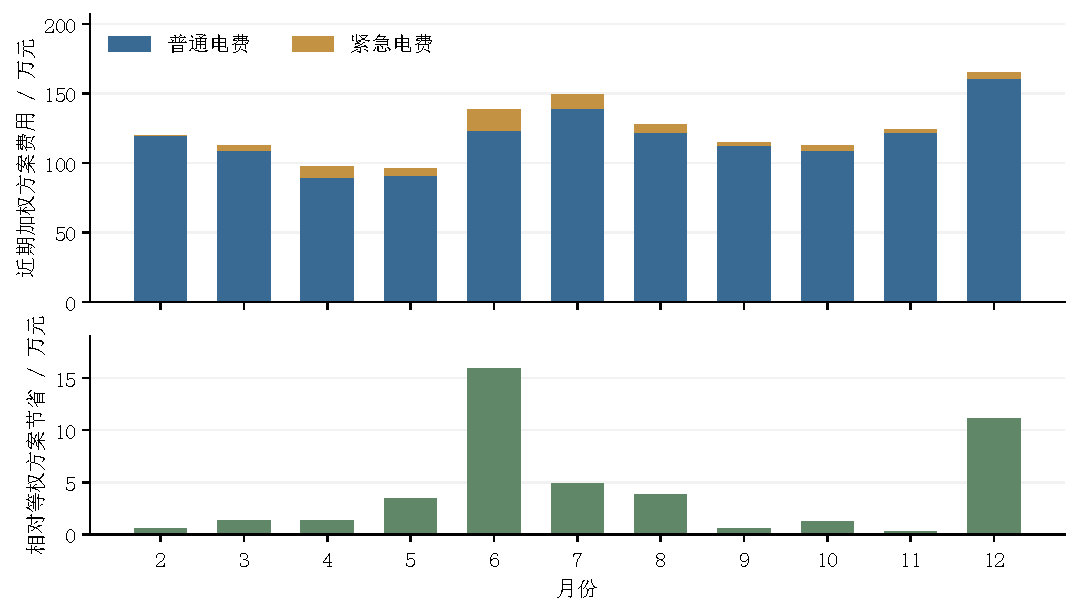
\includegraphics[width=.96\linewidth]{monthly_cost.pdf}
\caption{近期加权准备方案的月度费用及相对等权准备的节省}\label{fig:monthly}
\end{inlinefigure}
11个月合计均有所节省，但收益并不均匀，6月和12月贡献较多。这说明近期误差对订电的参考价值随供需变化而变化。月度节省也不代表每天更便宜：逐日比较中195天节省、135天增加、4天相同。6月3日最多节省32898.37元，6月24日则多支出19484.15元，反映出近期权重在减少缺口的同时也可能跟随短暂波动而多订电。

按题目指定日期，表\ref{tab:purchase}列出六个10分钟区间的计划购电量，以及全天购电和费用。各日总量取完整144段合计，不能由展示的六段相加代替。普通订单即使未实际利用也计入购电量和费用，紧急补购另列后汇总。
\begin{inlinetable}
\caption{指定日期的计划购电及全天费用（电量单位：kWh）}\label{tab:purchase}
\begin{tabular}{lrrrr}\toprule
区间或项目 & 3月20日 & 6月21日 & 9月23日 & 12月21日\\\midrule
\tableinput{tables/purchase.tex}
\bottomrule\end{tabular}
\end{inlinetable}

储能的实际运行见表\ref{tab:storage}。充放电量按设备外侧计量，日首尾库存按设备内部计量，两者通过90\%的充、放效率衔接。一个4小时区间内既有充电又有放电，是因为不同10分钟段采取了不同动作，并不表示同段同时充放。
\begin{inlinetable}
\caption{指定日期的实际充放电量及日首尾储电量（kWh）}\label{tab:storage}
\begin{tabular}{llrrrr}\toprule
区间 & 项目 & 3月20日 & 6月21日 & 9月23日 & 12月21日\\\midrule
\tableinput{tables/storage.tex}
\bottomrule\end{tabular}
\end{inlinetable}

四个指定日期中，两天发生紧急购电，时间、电量和费用见表\ref{tab:emergency}。6月21日和12月21日无紧急补购，说明供需预测存在偏差时，也可能由普通电和电池共同消化。
\begin{inlinetable}
\caption{指定日期的紧急购电}\label{tab:emergency}
\begin{tabular}{llrr}\toprule
日期 & 发生区间 & 电量 / kWh & 费用 / 元\\\midrule
\tableinput{tables/emergency.tex}
\bottomrule\end{tabular}
\end{inlinetable}

为说明电池怎样缓冲偏差，从题目指定日期中选取有紧急补购的3月20日和无紧急补购的6月21日，见图\ref{fig:days}。上图对照供需和订单，中图追踪实际库存，下图显示普通电之后的缺口由谁补齐。
\begin{inlinefigure}
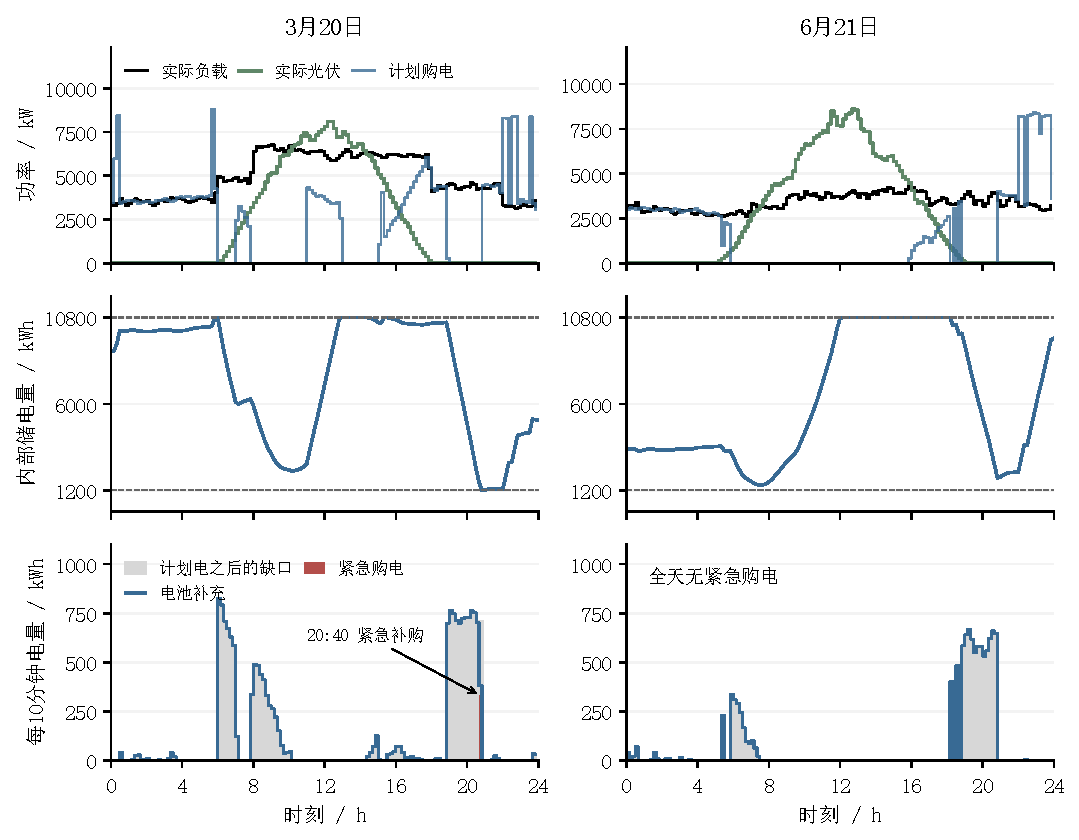
\includegraphics[width=.98\linewidth]{specified_days.pdf}
\caption{两个指定日期的供需、库存与缺口补充；虚线为储电上下限}\label{fig:days}
\end{inlinefigure}
3月20日的大部分缺口由电池补充，但20:40开始时内部库存仅1622.06 kWh，补电后达到1200 kWh下限，剩余329.52 kWh只能紧急购入。6月21日则通过白天吸收光伏和跨时段放电，全天未发生紧急补购。两天的差别说明，判断能否按时供电，需要同时看每段缺口、电池剩余电量和放电能力；全天总电量够用并不足以作出判断。这两个日期用于解释运行过程，全年优劣仍由完整334天比较确定。

\subsection*{8\quad 灵敏度检验与风险分析}

准备量是否越大越好，需要看多付的普通电费能否换来更多的紧急费下降。图\ref{fig:sensitivity}分别改变分位位置 $\alpha$ 和衰减参数 $\beta$，其余设置保持不变，费用变化均以 $\alpha=\beta=0.7$ 为参照。
\begin{inlinefigure}
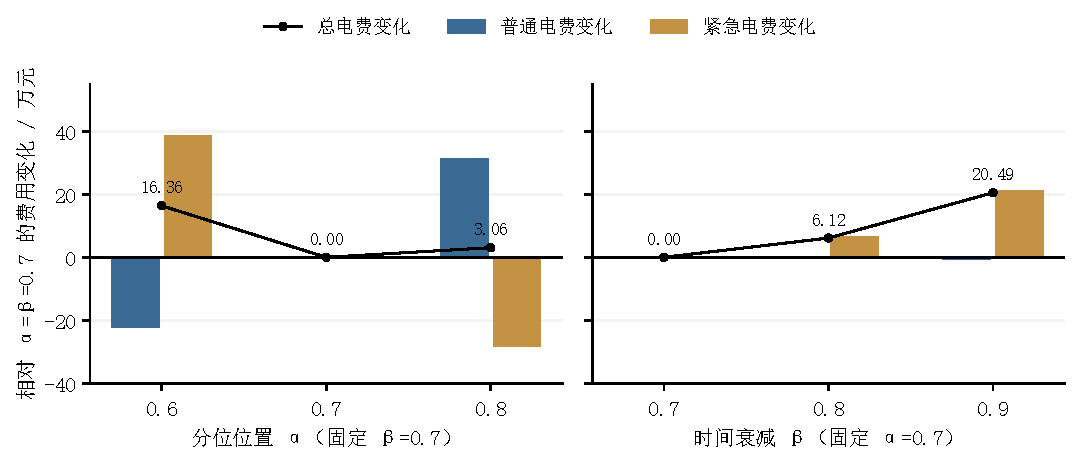
\includegraphics[width=.97\linewidth]{sensitivity.pdf}
\caption{准备程度与近期权重的费用影响（2025年2--12月）}\label{fig:sensitivity}
\end{inlinefigure}
将 $\alpha$ 从0.7提高到0.8后，紧急购电天数由156天降至102天，但普通电费的增加超过紧急电费的减少，总费用反而增加约3.06万元；降到0.6时，准备不足使总费增加约16.36万元。$\beta$ 从0.7提高到0.8或0.9后，旧误差保留更久，本次费用分别增加约6.12万元和20.49万元。因此，所试设置支持保留0.7附近的准备程度和较快的近期反应，并不证明连续参数范围内存在唯一最优点。

规划长度也有取舍。改为只看24小时后，总费用低3215.61元，差异约0.024\%，但紧急购电天数增加，最长连续紧急补购由200分钟延长至340分钟，年末库存也明显减少。故保留48小时是费用相近时对跨日库存和紧急风险的权衡。去掉式\eqref{eq:objective}的期末参考价值后，本次实际总费用未变，不能将它单独视作已证实的节费来源。

逐段复核了预测可用信息、电量平衡、设备限制、跨日库存和费用，结果相互一致。方案仍有156天需要紧急购电。其中，有的时段已达到最低库存，有的则受到放电功率限制，说明储能能够缓冲偏差，却无法消除全部预测风险。

为考察连续偏差是否会改变选择，再用过去已有的三天误差片段，分别构造持续低估负载、高估光伏及二者同时发生的情景。\footnote{每14天安排一次三天情景，从此前28天合格片段中按不利误差的90\%最近秩选取；该日程和排序位置均不表示真实发生概率。负载及联合情景实际扰动各45天，光伏72天；部分月份缺少合格片段，未额外补造扰动。}三类所测情景下，总费用仍比等权方案低3.09\%--3.52\%，说明近期准备的总体节费作用在这些偏差下得以保留。但短时波动也可能使其多订电，单日仍会失利。以上结论来自一个年份，方法选择也参考过全年诊断，因此支持本题数据下的应用，尚不足以保证在新年份或其他小区同样有效。

\end{document}
